\documentclass[12pt,a4paper]{article}

\usepackage[spanish]{babel} 
\usepackage[utf8]{inputenc}
\usepackage[numbers,sort&compress]{natbib} 
\usepackage{graphicx} 
\usepackage{amsfonts}
\usepackage[left=2cm,right=2cm,top=2cm,bottom=2cm]{geometry}
\usepackage{listings}
\usepackage[usenames,dvipsnames]{color}
\usepackage{setspace}

\lstset{ 
  language=R,
  basicstyle=\scriptsize\ttfamily,
  numbers=left,
  numberstyle=\tiny\color{Blue},
  stepnumber=1,
  numbersep=5pt,
  backgroundcolor=\color{white},
  showstringspaces=false,
  showtabs=false,
  frame=single,
  rulecolor=\color{black},
  tabsize=2,
  captionpos=b,
  breaklines=true,
  breakatwhitespace=false,        
  keywordstyle=\color{RoyalBlue},
  commentstyle=\color{YellowGreen},
  stringstyle=\color{ForestGreen}
}

\title{Matemáticas Computacionales \\ Práctica 3: Método de Bisección}
\author{1904381 Itzel Guadalupe Vega Yañez \\ Semestre Febrero - Junio 2021} 
\date{24 de Marzo del 2021}
\begin{document}

\maketitle

\section{Introducci\'{o}n}\label{sec:intro}

\onehalfspacing
En esta práctica 3 se implementa un método de Análisis Numérico para determinar los ceros de una función. En general, encontrar los ceros de una función en un número finito pasos casi nunca es posible. Para ello se utilizan métodos de aproximación. Estos métodos son iterativos iniciando con una aproximacón $x_{0}$ o un intervalo [$a, b$], calculamos aproximaciones sucesivas $x_{1}, x_{2},..., x_{n}$ y se escoge $x_{n}$ como aproximación del cero de la función cuando se cumpla un criterio de paro.

El método de bisección es uno de los métodos mas usuales.\citep{metodosnumericos}

\section{El m\'{e}todo de Bisecci\'{o}n} \label{sec:metodobiseccion}

\onehalfspacing
Este es uno de los métodos más sencillos y de fácil intuición, para resolver ecuaciones en una variable. Se basa en el Teorema de los Valores Intermedios, el cual establece que toda función continua $f$ en un intervalo cerrado [$a,b$] ($f \epsilon C[a,b]$) toma todos los valores que se hallan entre $f(a)$ y $f(b)$. Esto es, que todo valor entre $f(a)$ y $f(b)$ es la imagen de al menos un valor en el intervalo [$a,b$]. 





El método consiste en lo siguiente: Supongamos que en el intervalo [$a,b$] hay un cero de $f$. Calculamos el punto medio $m=\frac{a+b}{2}$ del intervalo [$a,b$] A continuación calculamos $f(m)$. En caso de que $f(m)$ sea igual a cero, ya hemos encontrado la solución buscada. En caso de que no lo sea, verificamos si $f(m)$ tiene signo opuesto al de $f(a)$. Se redefine el intervalo [$a,b$] como [$a,m$] o [$m,b$] según se haya determinado en cuál de estos intervalos ocurre un cambio de signo. A este nuevo intervalo se le aplica el mismo procedimiento y así, sucesivamente, iremos encerrando la solución en un intervalo cada vez más pequeño, hasta alcanzar la precisión deseada.\citep{repositorio}

En la siguiente figura se ilustra el procediemiento descrito
 \begin{figure}
 \centering
 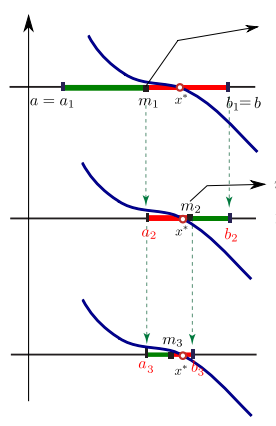
\includegraphics [ width =0.4\textwidth ]{ Grafi.png}
 \end{figure}
 \begin{equation}
		m_{1}=\frac{a_{1}+b_{1}}{2}, m_{1}\approx x^*
		Error\leq \frac{b-a}{2} = \frac{b_{1}-a_{1}}{2} 
		Actualizacion: f(a_{1})\cdot f(m_{1})>0\Longrightarrow \{ a_{2}=m_{1}, b_{2}=b_{1}
	\end{equation} 
	\begin{equation}
		m_{2}=\frac{a_{2}+b_{2}}{2}, m_{2}\approx x^*
		Error\leq \frac{b-a}{2^2} = \frac{b_{1}-a_{1}}{2} 
		Actualizacion: f(a_{2})\cdot f(m_{2})<0\Longrightarrow \{ a_{3}=a_{2}, b_{3}=m_{2}
	\end{equation} 



\subsection{Estimaci\'{o}n del error} \label{subsec:estimaciondelerror}
\onehalfspacing
El error exacto en el k-ésimo paso es $|m_{k}-x^*|$. Geométricamente se puede ver que esto es menos que la mitad del intervalo [$a_{k},b_{k}$], es decir,
\begin{equation}
|m_{k}-x^*|\leq \frac{ b_{k}-a_{k}}{2}= \frac{b-a}{2^k};
\end{equation}

\begin{enumerate}
		\item Resuelva $x^3=0$ usando bisección con el intervalo [$-0.2,0.1$]
		\item Resuelva $f=x^5-100x^4+3995x^3-79700x^2+794004x-3160075$ usando bisección con [$17,22.2$]
		\item Resuelva $x^3-2x-5=0$ 
\end{enumerate}


\begin{figure}
	\centering                                         
	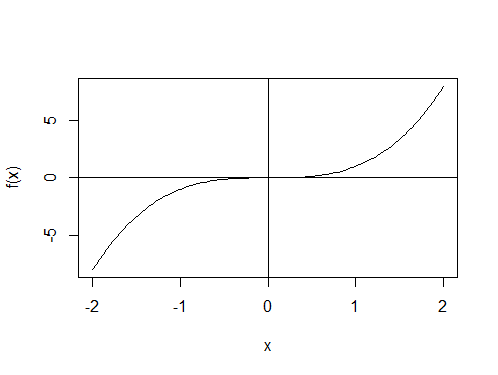
\includegraphics[scale = 1.0]{Ec1.png} 
	\caption{Grafica  $x^3=0$}           
\end{figure}

\begin{figure}
	\centering                                         
	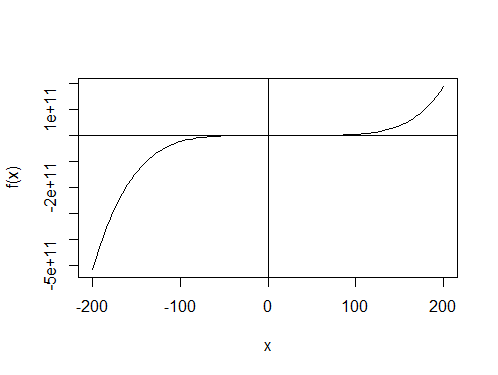
\includegraphics[scale = 1.0]{Ec2.png} 
	\caption{Grafica  $f=x^5-100x^4+3995x^3-79700x^2+794004x-3160075$}            
\end{figure}

\bibliography{biblio}
\bibliographystyle{plainnat}


\end{document}
